\section{Experiments}
\label{sec:experiments}

\subsection{Datasets}
\label{sec:datasets}

We evaluate on three benchmarks chosen to span the spectrum of construction artifact severity.
\textbf{CIFAKE}~\cite{cifake} contains 10k real (CIFAR-10) and 10k fake (Stable Diffusion v1.4) test images, both downsampled to $32\times32$ JPEG --- no format or resolution bias.
\textbf{Defactify}~\cite{defactify} has 7.5k real and 37.5k fake JPEG test images; all images share the same format, but fake images have only 5--6 unique resolutions (canonical AI output sizes) vs.\ 180+ for real images --- resolution bias, no format bias.
\textbf{GenImage}~\cite{genimage} uses 50k real ImageNet photographs (JPEG, hundreds of unique resolutions) and 76,677 ADM-generated fake images (PNG, uniform $256\times256$) --- simultaneous severe format and resolution bias.
All six external detectors were trained on ProGAN/ForenSynths~\cite{wang2020cnn}, which has the same JPEG=real/PNG=fake construction as GenImage; all three test sets are therefore out-of-distribution.

\subsection{Act 1: Spectral Bias in the Data}
\label{sec:audit}

\begin{figure}[t]
  \centering
  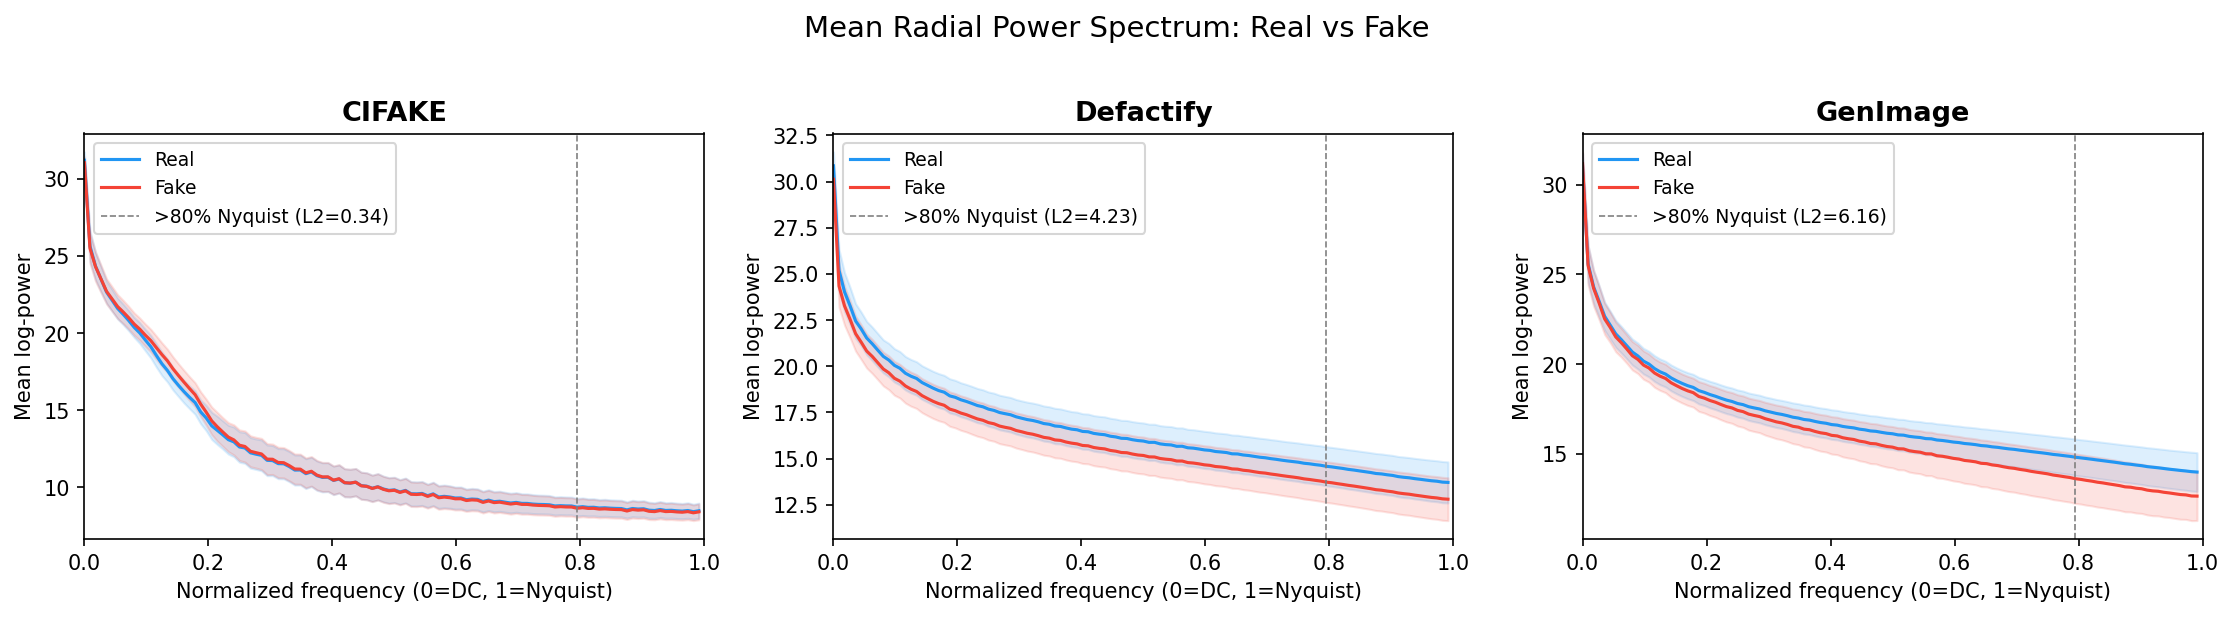
\includegraphics[width=\linewidth]{fig1_radial_spectra.png}
  \caption{Mean radial log-power spectra for real vs.\ fake splits across all three datasets (original, unmodified data). Shaded regions: $\pm1\sigma$. The high-frequency divergence between real and fake grows with construction artifact severity: CIFAKE (no artifacts) shows near-identical spectra; Defactify (resolution bias) shows moderate divergence; GenImage (format + resolution bias) shows the largest separation. HF L2 divergence values: CIFAKE $=0.34$, Defactify $=4.23$, GenImage $=6.16$.}
  \label{fig:spectra}
\end{figure}

\begin{table}[t]
\centering
\small
\begin{tabular}{lccc}
\toprule
\textbf{Dataset} & \textbf{Format bias} & \textbf{Resolution bias} & \textbf{HF-L2} \\
\midrule
CIFAKE    & None         & None        & 0.34 \\
Defactify & None         & \textbf{Severe}  & 4.23 \\
GenImage  & \textbf{Severe} & \textbf{Severe} & 6.16 \\
\bottomrule
\end{tabular}
\caption{Dataset audit summary. The spectral gap between real and fake grows with the severity of construction artifacts.}
\label{tab:audit}
\end{table}
Figure~\ref{fig:spectra} and Table~\ref{tab:audit} establish the first part of the story. CIFAKE, the only artifact-controlled benchmark in our set, has almost no spectral separation between real and fake. Defactify shows a much larger gap, and GenImage is larger still. The ordering is exactly what we would expect if format and resolution mismatches are producing easy-to-learn frequency shortcuts before a detector sees any semantic content.

\paragraph{Trivial format baseline.}
As a zero-parameter lower bound, we classify images by file extension alone: PNG $\to$ fake, JPEG $\to$ real. On CIFAKE and Defactify, where both classes share the same format, this achieves exactly AUC $= 0.500$. On GenImage, it achieves AUC $= 1.000$ --- perfect separation before any model is involved. The format shortcut in GenImage is not merely present; it is sufficient.

\subsection{Act 2: Detector Performance on Original Benchmarks}
\label{sec:baseline}

\begin{table}[t]
\centering
\small
\setlength{\tabcolsep}{4pt}
\begin{tabular}{lcccc}
\toprule
\textbf{Detector} & \textbf{CIFAKE} & \textbf{CIFAKE-N} & \textbf{Defactify} & \textbf{Defactify-N} \\
\midrule
CNNDetection~\cite{wang2020cnn} & 0.375 & 0.375 & 0.507 & 0.524 \\
FreqNet~\cite{freqnet}          & 0.473 & 0.473 & 0.511 & 0.534 \\
NPR~\cite{npr}                  & 0.435 & 0.435 & 0.520 & 0.556 \\
UnivFD~\cite{univfd}            & 0.300 & 0.371 & 0.536 & 0.493 \\
FatFormer~\cite{fatformer}      & 0.290 & 0.290 & 0.557 & 0.537 \\
B-Free~\cite{bfree}             & 0.497 & \textbf{0.637} & 0.611 & \textbf{0.611} \\
CNN2D (ours)                    & 0.530 & 0.472 & 0.546 & 0.537 \\
\bottomrule
\end{tabular}
\caption{Completed AUC results on original and normalized test sets. Normalization converts all images to $256\times256$ PNG. CIFAKE-N and Defactify-N are normalized variants.}
\label{tab:perf}
\end{table}

Table~\ref{tab:perf} contains the central negative result. On CIFAKE, every external detector is below chance. This is stronger than saying that the models do not generalize. AUCs of $0.375$, $0.473$, $0.435$, $0.300$, $0.290$, and $0.497$ imply that the detectors often rank real images as more fake than fake images. We interpret this as evidence of an inverted rule learned from biased training conditions.

The contrast with Defactify is also useful. Defactify contains measurable bias, but it is mostly a resolution bias, not the JPEG/PNG pattern that dominates GenImage. All six detectors stay near chance on both the original and normalized versions of Defactify (AUC 0.507--0.611). The exception is B-Free, which reaches 0.611 on both original and normalized Defactify; we discuss this separately in Section~\ref{sec:norm_results}. The key result is that resolution bias alone does not trigger the same shortcut as format bias. Benchmark success depends on whether the test set reproduces the particular shortcut the detector has learned.

\subsection{Act 2 (cont.): Effect of Normalization}
\label{sec:norm_results}

\noindent\textbf{CIFAKE after normalization.}
Most detectors do not move at all: CNNDetection, FreqNet, NPR, and FatFormer have identical AUC before and after normalization. This implies that their failure on CIFAKE is not tied to file metadata alone. The misleading cue is already embedded in the pixels, likely through the blocky appearance of heavily compressed $32\times32$ natural images.

\noindent\textbf{The B-Free exception.}
B-Free is the only detector that clearly improves after normalization, rising from $0.497$ to $0.637$ on CIFAKE and reaching $0.611$ on normalized Defactify. This suggests a different operating regime: once format confounds are reduced, B-Free's DINOv2-based features can use visual quality differences that the frequency-heavy models do not exploit reliably.

\noindent\textbf{Interpretation.}
The normalization results are not a full deconfounding study, but they do separate two behaviors. Most detectors remain shortcut-bound even after re-encoding. B-Free benefits from cleaner inputs. That contrast is useful because it shows the story is not simply ``all detectors fail.'' The more specific result is that most current detectors appear to depend on brittle benchmark cues, while at least one model seems partially sensitive to something more robust.

\subsection{Act 3: Shortcut Transfer on GenImage}
\label{sec:genimage_results}

\begin{table}[t]
\centering
\small
\begin{tabular}{lcccc}
\toprule
\textbf{Detector} & \textbf{CIFAKE} & \textbf{GenImage} & \textbf{GenImage-N} & \textbf{$\Delta$(CIF$\to$GI)} \\
\midrule
CNNDetection~\cite{wang2020cnn} & 0.375 & 0.658 & 0.652 & $+0.283$ \\
FreqNet~\cite{freqnet}          & 0.473 & \textbf{0.977} & \textbf{0.978} & $+0.504$ \\
NPR~\cite{npr}                  & 0.435 & \textbf{0.951} & \textbf{0.940} & $+0.516$ \\
UnivFD~\cite{univfd}            & 0.300 & \textbf{0.961} & \textbf{0.940} & $+0.661$ \\
FatFormer~\cite{fatformer}      & 0.290 & \textbf{0.975} & \textbf{0.968} & $+0.685$ \\
B-Free~\cite{bfree}             & 0.497 & \textbf{0.919} & \textbf{0.919} & $+0.422$ \\
CNN2D (ours)                    & 0.530 & -- & 0.497 & -- \\
\bottomrule
\end{tabular}
\caption{AUC on CIFAKE, GenImage (original), and GenImage-N (normalized to $256\times256$ PNG), with per-detector swing from CIFAKE to GenImage. Normalization removes format and resolution artifacts. GenImage-N AUC barely changes ($\leq 0.02$ drop), confirming that high GenImage performance reflects genuine ADM generative artifacts rather than format shortcuts.}
\label{tab:genimage}
\end{table}

Table~\ref{tab:genimage} provides the strongest evidence for shortcut transfer. The jump from CIFAKE to GenImage is dramatic: FatFormer improves by $+0.685$, UnivFD by $+0.661$, NPR by $+0.516$, FreqNet by $+0.504$, B-Free by $+0.422$, and CNNDetection by $+0.283$. All six external detectors move from below-chance or near-chance on the artifact-free benchmark to above $0.91$ on the shortcut-laden one. These are not small robustness fluctuations but rather regime changes driven by a single variable: whether the JPEG=real/PNG=fake pattern is accessible.

\noindent\textbf{GenImage after normalization.}
Normalizing GenImage to $256\times256$ PNG removes both format and resolution shortcuts, yet AUC changes by at most $0.02$ across all six detectors --- and B-Free's AUC is identical to four decimal places ($0.9194\to0.9194$, $\Delta=0.000$). This result sharpens the interpretation: high GenImage performance reflects genuine ADM spectral artifacts, not format shortcuts. The CIFAKE inversion therefore cannot be explained symmetrically as ``the same shortcut firing in reverse'' --- it reflects detectors trained on full-resolution JPEG naturals firing backward on heavily-compressed $32\times32$ CIFAR-10 images, a distribution shift in the real class, not the format. The two findings together define the diagnostic value of CIFAKE: it withholds both format shortcuts and easy generative signatures, forcing the inverted decision rule into the open.

\subsection{Act 4: Format-Swap as a Causal Probe}
\label{sec:swap_results}

\begin{table}[t]
\centering
\small
\setlength{\tabcolsep}{4pt}
\begin{tabular}{lcccc}
\toprule
 & \multicolumn{2}{c}{\textbf{CIFAKE}} & \multicolumn{2}{c}{\textbf{GenImage}} \\
\cmidrule(lr){2-3}\cmidrule(lr){4-5}
\textbf{Detector} & Original & Swapped & Original & Swapped \\
\midrule
CNNDetection~\cite{wang2020cnn} & 0.375 & 0.354 & 0.658 & 0.609 \\
FreqNet~\cite{freqnet}          & 0.473 & 0.453 & 0.977 & 0.503 \\
NPR~\cite{npr}                  & 0.435 & 0.436 & 0.951 & 0.381 \\
UnivFD~\cite{univfd}            & 0.300 & 0.298 & 0.961 & 0.930 \\
FatFormer~\cite{fatformer}      & 0.290 & 0.272 & 0.975 & 0.811 \\
B-Free~\cite{bfree}             & 0.497 & 0.619 & 0.919 & -- \\
CNN2D (ours)                    & 0.530 & \textbf{0.969} & 0.497$^\dag$ & \textbf{0.998} \\
\bottomrule
\end{tabular}
\caption{Format-swap results (AUC). All real images are re-encoded as PNG; all fake images as JPEG at quality~85, reversing the natural format association. CIFAKE originally has no format bias; GenImage has near-total format bias. $^\dag$~CNN2D GenImage evaluated on the normalized split (no original checkpoint exists).}
\label{tab:swap}
\end{table}

Table~\ref{tab:swap} provides the sharpest causal test in this paper. The logic is simple: if format is the mechanism, reversing it should reverse the performance.

\noindent\textbf{On CIFAKE}, where both classes are JPEG in the original data, introducing a format difference produces negligible change for five of the six external detectors. They were not exploiting a format shortcut on CIFAKE because none existed; swapping formats does not create one they can read. CNN2D is the exception: when fake images are re-JPEG-compressed at $32\times32$ and real images are losslessly re-encoded as PNG, CNN2D jumps from $0.530$ to $0.969$. Repeated JPEG compression of small images introduces quantization noise that the spectral CNN can exploit once it is class-specific. B-Free also improves modestly ($0.497\to0.619$), consistent with its earlier normalization result suggesting sensitivity to image quality differences.

\noindent\textbf{On GenImage}, the reversal is decisive for two models. FreqNet drops from $0.977$ to $0.503$ --- chance --- after the format swap. NPR drops from $0.951$ to $0.381$, inverting below chance. For these two detectors, format was not merely helpful; it was the primary driver. CNNDetection drops modestly ($0.658\to0.609$). UnivFD and FatFormer retain substantial performance ($0.930$ and $0.811$), suggesting a mixture of format shortcuts and genuine ADM-specific content. CNN2D, near chance on normalized GenImage ($0.497$), reaches $0.998$ on format-swapped GenImage: making fakes look like compressed natural images gives our CIFAKE-trained model exactly the cue it was trained on.

The CIFAKE and GenImage results are jointly consistent: external detectors do not react to format changes when no format shortcut was accessible (CIFAKE), and collapse or invert when the shortcut they relied on is reversed (GenImage).

\subsection{Act 5: Frequency Band Ablation}
\label{sec:ablation_results}

\begin{table}[t]
\centering
\small
\setlength{\tabcolsep}{5pt}
\begin{tabular}{lcccc}
\toprule
\textbf{Detector} & \textbf{Original} & \textbf{Low rem.} & \textbf{Mid rem.} & $\boldsymbol{\Delta}_\text{low}$ \\
\midrule
CNNDetection~\cite{wang2020cnn} & 0.658 & 0.601 & 0.601 & $-0.06$ \\
FreqNet~\cite{freqnet}          & 0.977 & 0.636 & 0.933 & $-0.34$ \\
NPR~\cite{npr}                  & 0.951 & 0.391 & 0.509 & $-0.56$ \\
UnivFD~\cite{univfd}            & 0.961 & 0.559 & --    & $-0.40$ \\
FatFormer~\cite{fatformer}      & 0.975 & 0.680 & --    & $-0.30$ \\
B-Free~\cite{bfree}             & 0.919 & 0.578 & --    & $-0.34$ \\
CNN2D (ours)                    & 0.497$^\dag$ & 0.807 & 0.901 & $+0.31$ \\
\bottomrule
\end{tabular}
\caption{Band ablation on GenImage (normalized), AUC. Low band: $r < 0.2\,r_{\max}$; Mid band: $0.2\leq r < 0.6\,r_{\max}$. High-band results are pending for all detectors; mid-band results are pending for UnivFD, FatFormer, and B-Free. $^\dag$~CNN2D normalized baseline.}
\label{tab:ablation}
\end{table}

Table~\ref{tab:ablation} localizes the shortcut to the low-frequency regime. Removing the low-frequency band ($r < 0.2\,r_{\max}$) causes the largest AUC drop for every external detector on GenImage: NPR falls by $-0.56$, UnivFD by $-0.40$, FreqNet by $-0.34$, and B-Free by $-0.34$. The low band captures the dominant energy of JPEG blocking artifacts and the global intensity statistics that differ when one class is uniformly JPEG and the other is uniformly PNG --- exactly where the GenImage shortcut lives.

Removing the mid-frequency band is substantially less damaging. FreqNet recovers to $0.933$ under mid-band ablation, indicating that its remaining signal lives mostly in mid frequencies once low-frequency content is present. NPR, which was already inverted under low-band removal, stays suppressed at $0.509$ under mid-band removal --- consistent with it having no reliable signal beyond the low-frequency format cue.

On CIFAKE, where external detectors were already near chance, band ablation produces less coherent changes, as expected: there is no shortcut to remove. Two results stand out. FatFormer, which scored $0.290$ on original CIFAKE, jumps to $0.692$ when the low-frequency band is removed. The low-frequency content in CIFAKE's heavily-compressed $32\times32$ images was actively suppressing FatFormer's performance --- removing it reveals a modest latent signal. CNN2D improves on all three ablations (low: $0.661$, mid: $0.787$, high: $0.753$), with the largest improvement from mid-band removal. On Defactify, which has resolution bias but no format bias, all detectors remain near chance across all bands, consistent with the absence of the specific shortcut these models learned.

\noindent\textbf{Summary.}
The format-swap and band ablation results close the causal loop opened in Acts 1--3. The bias exists in the data (Act~1); detectors fail without it (Act~2); they succeed when it reappears (Act~3); swapping it reverses their performance (Act~4); and ablating the low-frequency band --- where format artifacts concentrate --- destroys their advantage (Act~5). Each step tightens the case that format artifacts are the operative mechanism, not a confounding correlation.
